\chapter{Introducción} % Introducción
\hyphenation{In-te-re-se}
\section{Contexto y motivación del proyecto} % Contexto y motivación del proyecto
La adopción de las tecnologías inalámbricas para la transmisión y comunicación de datos aumenta cada día. El auge de la domótica, los sistemas IoT (del inglés Internet of Things) y el comienzo de la adopción de los dispositivos \textit{wearables}, auguran un largo futuro tanto a los protocolos y tecnologías existentes como a la creación de nuevos sistemas y protocolos de comunicación inalámbricos.
\\Un aspecto que se debe abordar para la comunicación de estos dispositivos es el de la seguridad, implementando los mecanismos para garantizar la fiabilidad y confidencialidad de las comunicaciones, así como prevenir accesos no autorizados a los dispositivos de manera remota.
\\\\
Dentro de estas tecnologías de comunicación inalámbrica como pueden ser \textit{wifi} o \textit{bluetooth}, destacan otras menos populares que están cobrando notoriedad en entornos domésticos e industriales debido a sus características más novedosas. Entre estas tecnologías se encuentran los protocolos Thread y Zigbee.
\\\\Thread es un protocolo de comunicación inalámbrica de baja potencia construido con 6LowPan \cite{especificacionthread} y diseñado para permitir la comunicación de manera fácil y segura y el transporte de datos IPV6 entre dispositivos IoT. Mientras que Zigbee es un protocolo de comunicación inalámbrica para la radiodifusión digital de datos diseñado para permitir el control y la monitorización de dispositivos conectados, proporcionando una tasa de envío de datos baja y priorizando la vida útil de las baterías. Las características de Thread y Zigbee los hacen unos protocolos idóneos para su uso en dispositivos y redes IoT, así como para todo aquel dispositivo que necesite una conectividad de larga duración debido a su poco consumo.
\\\\
Con la motivación de profundizar más en estas tecnologías, su funcionamiento y principalmente su seguridad, se ha llevado a cabo un proyecto mediante el cual evaluar el estado del arte de las comunicaciones IoT, los mecanismos de identificación de dispositivos y los ataques a los protocolos y a las tecnologías IoT.
\clearpage




\section{Objetivos del proyecto} % Objetivos del proyecto
\vspace{0.5cm}
El objetivo principal que se persigue con la realización de este proyecto es el siguiente:
\begin{itemize}
\item Ofrecer una visión actualizada del nivel de seguridad existente en las redes IoT y en especial en las redes inalámbricas Thread y Zigbee, basada en la investigación del estado del arte de la seguridad, así como la revisión de las técnicas disponibles para llevar a cabo tanto ataques como contramedidas a los protocolos de IoT.
\end{itemize}
\vspace{0.7cm}

Para conseguir este objetivo general, se deben de llevar a cabo otros de aspecto más específico:
\begin{itemize}
\item Realizar un análisis de las características y los modelos de comunicación entre dispositivos IoT.
\item Analizar los diferentes protocolos de comunicación IoT (Wifi, Cellular, Sigfox, Z-wave, …).
\item Realizar un estudio completo del estándar IEEE 802.15.4, y los protocolos Thread y Zigbee, así como del funcionamiento de sus comunicaciones inalámbricas.
\item Analizar las vulnerabilidades y ataques recientes contra las tecnologías de IoT.
\item Llevar a cabo una auditoría de seguridad inalámbrica sobre una red industrial Zigbee, siguiendo la metodología OWISAM.
\item Documentar y detallar las medidas preventivas y/o correctivas que se deberían de establecer para mejorar la seguridad en las redes IoT.
\end{itemize}
\clearpage




\section{Glosario de Términos} % Glosario de términos
A continuación, se presenta una lista de términos del proyecto con sus respectivas definiciones que se usarán a lo largo del documento. Por este motivo se recomienda la lectura de estos antes de proceder con el resto del documento.
\begin{itemize}
\item{\bf IoT}: concepto referido a escenarios donde la conectividad de
red y la capacidad informática se extiende a objetos, sensores y elementos cotidianos.
\item{\bf Domótica}: concepto referido a sistemas capaces de automatizar una vivienda o edificación, aportando servicios de gestión energética, seguridad, etc.
\item{\bf WPAN}: tipo de red personal que utiliza tecnologías de comunicación inalámbrica para comunicarse y transferir datos entre los dispositivos conectados.
\item{\bf Auditoría de seguridad}: evaluación del nivel de madurez en seguridad en un determinado ámbito, donde se analizan las políticas y procedimientos implementados así como las medidas técnicas, permitiendo detectar debilidades y vulnerabilidades.
\item{\bf CoaP (Constrained Application Protocol)}: protocolo de capa de servicio diseñado para su uso en dispositivos de Internet con recursos limitados, como nodos de redes de sensores inalámbricos.
\item{\bf Bandas ISM}: bandas de radio reservadas internacionalmente para el uso de radiofrecuencias con fines industriales, científicos y médicos.
\item{\bf CSMA/CA}: método de acceso múltiple a una red, donde los nodos intentan evitar colisiones iniciando la transmisión después de que se detecta que el canal está ''libre''.
\item{\bf DTLS (Datagram Transport Layer Security)}: protocolo de comunicaciones que proporciona seguridad para aplicaciones basadas en datagramas, evitando escuchas o manipulaciones de mensajes.
\item{\bf Exploit-DB}: base de datos mundial sobre exploits y brechas de seguridad donde se publican vulnerabilidades de aplicaciones e instrucciones para aprovecharse de ellas.
\item{\bf PoC (Proof of Concept)}: demostración de un determinado método o teoría con el fin de mostrar su viabilidad.
\item{\bf CWE (Common Weakness Enumeration)}: lista desarrollada por la comunidad de tipos comunes de debilidades de software y hardware.
\end{itemize}




\clearpage

 


\section{Metodología} % Metodología seguida
Se ha optado por la utilización de la metodología OWISAM, puesto que es una metodología orientada a proyectos de investigación y análisis de seguridad en redes inalámbricas.
\\\\
OWISAM, acrónimo de Open Wireless Security Assessment Methodology, es una metodología ágil utilizada en auditorías de seguridad y test de intrusión, que ayuda a realizar con éxito un análisis sobre entornos de redes inalámbricas. Esta metodología fue creada para minimizar el impacto de los ataques informáticos y garantizar la protección de las infraestructuras Wireless basadas en el estándar IEEE 802.11 (Wi-Fi). Sin embargo, también se puede orientar a las tecnologías de IoT Thread y Zigbee, basadas en el estándar IEEE 802.15.4.
\\\\\\
De esta forma se aplicarán en el proyecto los controles y las fases del análisis de seguridad que especifica OWISAM, pero aplicadas a las tecnologías de IoT.
\\\\
\begin{figure}[H]
\centerline{\includegraphics[width=15cm]{figuras/metodologia_owisam.eps}}
\caption{Esquema de la metodología OWISAM \cite{metodologiaowisam}}
\label{metodologia-owisam}
\end{figure}
\clearpage




%\begin{landscape}
\section{Planificación del proyecto} % Planificación del proyecto
A continuación, se presenta la planificación seguida para este Trabajo Final de Grado, en la cual se recogen las tareas y los hitos más importantes del trabajo. La planificación inicial se ha ido modificando y adaptando conforme se profundizaba en el estudio de los protocolos Thread y Zigbee, y se analizaba su seguridad.
En consecuencia, la planificación final llevada a cabo es la que se recoge en el siguiente diagrama de Gantt:
\begin{figure}[H]
\centerline{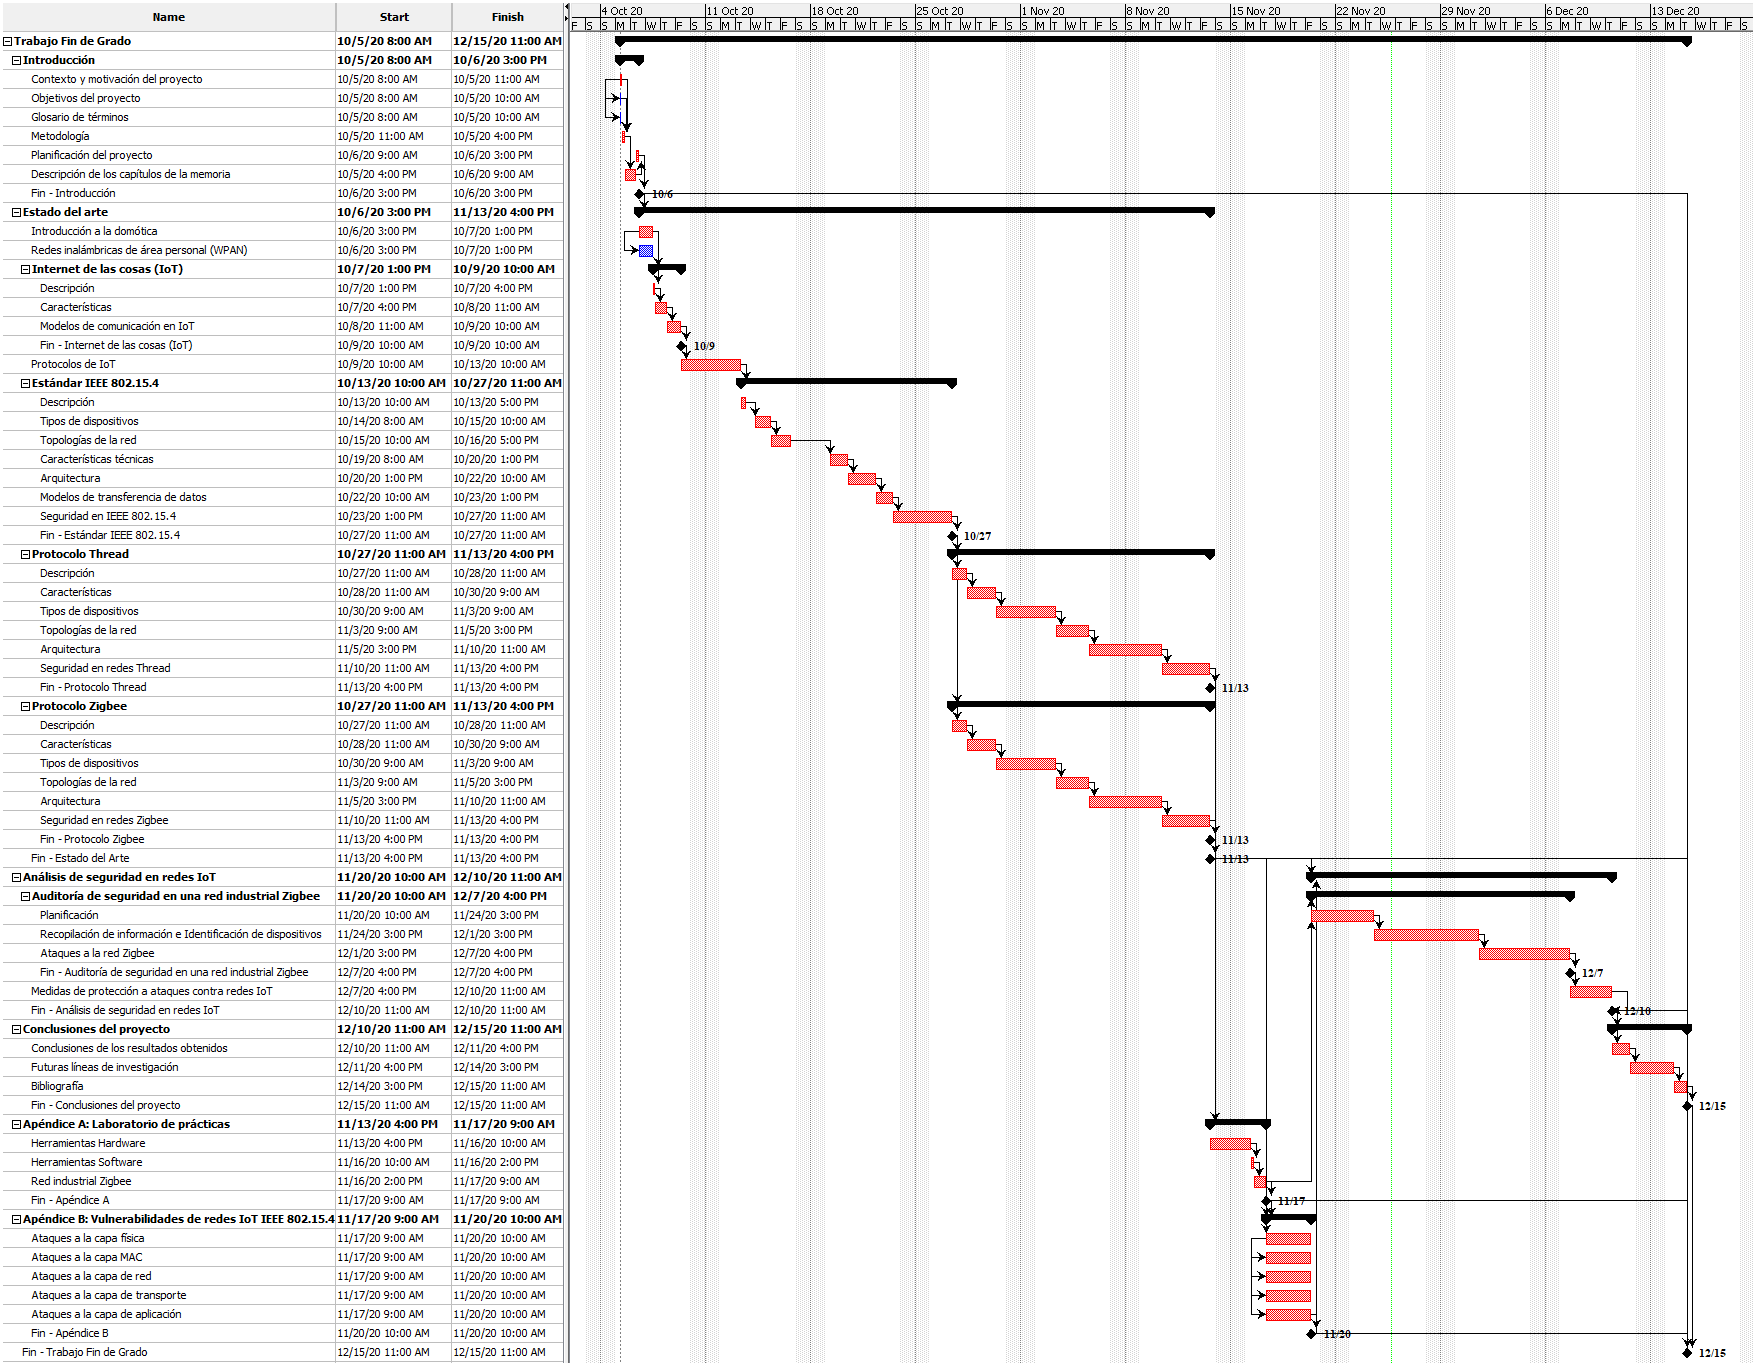
\includegraphics[width=19cm]{figuras/gantt.png}}
\caption{Planificación del proyecto}
\label{planificacion}
\end{figure}
%\end{landscape}
\clearpage



\section{Descripción de los capítulos de la memoria} % Breve descripción de los capítulos de la memoria
El presente documento se encuentra organizado en los siguientes 4 capítulos:
\begin{itemize}
\item{\bf Capítulo 1 - Introducción}: se presenta el proyecto, explicando su motivación y objetivos a perseguir. Además, se explica la metodología de análisis de seguridad a utilizar en  el proyecto, así como la planificación seguida para la realización del mismo.
\item{\bf Capítulo 2 - Estado del Arte}: es el capítulo central en el que se recopilan los detalles técnicos sobre los que se apoya el estudio. Se realiza una introducción al ámbito del internet de las cosas (IoT) y se explica de forma detallada y completa el funcionamiento del estándar IEEE 802.15.4 y de los protocolos Thread y Zigbee (características, tipos de dispositivos, topología de red, arquitectura, medidas de seguridad, ...).
\item{\bf Capítulo 3 - Análisis de seguridad en redes IoT}: partiendo del estudio realizado en el capítulo anterior, se analizan las debilidades y las vulnerabilidades de la redes IoT basadas en el estándar IEEE 802.15.4, explicando los ataques existentes y las contramedidas a implementar. Posteriormente, se realiza una auditoría de seguridad en la red IoT de un entorno industrial que implementa el protocolo Zigbee, descubriendo y publicando en Exploit-DB una vulnerabilidad desconocida hasta el momento en los dispositivos Zigbee del fabricante Ksix, que permite falsificar mensajes entre dispositivos de forma remota.
\item{\bf Capítulo 4 - Conclusiones del proyecto}: se exponen los resultados y las conclusiones finales de la investigación y de las tecnologías de IoT analizadas (IEEE 802.15.4, Thread y Zigbee) y su seguridad.
\end{itemize}
